                %%%%%%%%%%%%%%%%%%%%%%%%%%%%%%%%%%%%%%%%%
% Beamer Presentation
% LaTeX Template
% Version 1.0 (10/11/12)
%
% This template has been downloaded from:
% http://www.LaTeXTemplates.com
%
% License:
% CC BY-NC-SA 3.0 (http://creativecommons.org/licenses/by-nc-sa/3.0/)
%
%%%%%%%%%%%%%%%%%%%%%%%%%%%%%%%%%%%%%%%%%

%----------------------------------------------------------------------------------------
%   PACKAGES AND THEMES
%----------------------------------------------------------------------------------------

\documentclass{beamer}

\mode<presentation> {

% The Beamer class comes with a number of default slide themes
% which change the colors and layouts of slides. Below this is a list
% of all the themes, uncomment each in turn to see what they look like.

%\usetheme{default}
%\usetheme{AnnArbor}
%\usetheme{Antibes}
%\usetheme{Bergen}
%\usetheme{Berkeley}
%\usetheme{Berlin}
%\usetheme{Boadilla}
%\usetheme{CambridgeUS}
%\usetheme{Copenhagen}
%\usetheme{Darmstadt}
%\usetheme{Dresden}
%\usetheme{Frankfurt}
%\usetheme{Goettingen}
%\usetheme{Hannover}
%\usetheme{Ilmenau}
%\usetheme{JuanLesPins}
%\usetheme{Luebeck}
\usetheme{Madrid}
%\usetheme{Malmoe}
%\usetheme{Marburg}
%\usetheme{Montpellier}
%\usetheme{PaloAlto}
%\usetheme{Pittsburgh}
%\usetheme{Rochester}
%\usetheme{Singapore}
%\usetheme{Szeged}
%\usetheme{Warsaw}

% As well as themes, the Beamer class has a number of color themes
% for any slide theme. Uncomment each of these in turn to see how it
% changes the colors of your current slide theme.

%\usecolortheme{albatross}
%\usecolortheme{beaver}
%\usecolortheme{beetle}
%\usecolortheme{crane}
%\usecolortheme{dolphin}
%\usecolortheme{dove}
%\usecolortheme{fly}
%\usecolortheme{lily}
%\usecolortheme{orchid}
%\usecolortheme{rose}
%\usecolortheme{seagull}
%\usecolortheme{seahorse}
%\usecolortheme{whale}
%\usecolortheme{wolverine}

%\setbeamertemplate{footline} % To remove the footer line in all slides uncomment this line
%\setbeamertemplate{footline}[page number] % To replace the footer line in all slides with a simple slide count uncomment this line

%\setbeamertemplate{navigation symbols}{} % To remove the navigation symbols from the bottom of all slides uncomment this line
}

\usepackage{graphicx} % Allows including images
\usepackage{booktabs} % Allows the use of \toprule, \midrule and \bottomrule in tables
\usepackage{amsmath}
\usepackage{setspace}
\usepackage{biblatex}

%----------------------------------------------------------------------------------------
%   TITLE PAGE
%----------------------------------------------------------------------------------------

\title[Q-prop]{Baselines and ER in policy gradient learning} % The short title appears at the bottom of every slide, the full title is only on the title page

\author{Nikita Petrenko} % Your name

\date{\today} % Date, can be changed to a custom date

\begin{document}

\begin{frame}
\titlepage % Print the title page as the first slide
\end{frame}

\begin{frame}
\frametitle{Overview} % Table of contents slide, comment this block out to remove it
\tableofcontents % Throughout your presentation, if you choose to use \section{} and \subsection{} commands, these will automatically be printed on this slide as an overview of your presentation
\end{frame}

%----------------------------------------------------------------------------------------
%   PRESENTATION SLIDES
%----------------------------------------------------------------------------------------

%------------------------------------------------
\section{Overview of common policy gradient methods} % Sections can be created in order to organize your presentation into discrete blocks, all sections and subsections are automatically printed in the table of contents as an overview of the talk


\begin{frame}[t]
\frametitle{Common methods of PG learning}

Discounted state distribution: $\rho_\pi :=  (1-\gamma) \sum_{t=0}^\infty \gamma^t P(s_0 \rightarrow s | t)$ 

\begin{itemize}

\item A3C: $\nabla_\theta V(s) = E_{\rho_\pi, \pi}(\nabla \log \pi_\theta (a) * (r(s,a) + \gamma V(s') - V(s)))$ 
\\basic algorithm which exhibits high gradient variance and inability to learn on off-policy data (including Experience Replay)

\item A3C with Importance Sampling (IS): \[ \nabla_\theta V(s) = E_{traj \sim \pi_{\theta'}} \left[ \dfrac{P(traj)}{P'(traj)} \nabla \log \pi_\theta (a) (r(s,a) + \gamma V(s') - V(s)) \right] \]
\\Unbiased estimation of policy gradient with off-policy data. However, it suffers from possibly infinite variance of density ratios if behavioral policy (the one that collected samples) and agent policy are too different.
\\In MDP setting, 

\begin{equation}
\dfrac{P(traj)}{P'(traj)} = \dfrac{p(s_0) \pi (a_0 | s_0) p(s_1 | a_0, s_0)
...} {p(s_0) \pi' (a_0 | s_0) p(s_1 | a_0, s_0)
...} = \prod_{t=0}^{T-1} \dfrac{\pi (a_t | s_t)} {\pi' (a_t | s_t)}
\end{equation}

\end{itemize}
\end{frame}

\begin{frame}[t]
\frametitle{Common methods of PG learning}
\begin{itemize}

\item TRPO: derives lower bound on policy improvement thus allowing to make several gradient update steps on sampled trajectories. Improves sample efficiency significantly.

\end{itemize}
\end{frame}

%------------------------------------------------
\section{Q-prop}
%------------------------------------------------
\subsection{Features}

\begin{frame}[t]
\frametitle{Q-prop}

Main features:
\begin{itemize}
\item Unbiased, low variance gradient
\item On-policy actor with control variate
\item Off-policy critic
\item Ability to use TRPO for policy updates
\end{itemize}

\vspace{4mm}
Limitations:
\begin{itemize}
\item Continuous control only
\end{itemize}

\end{frame}

\subsection{Q-prop estimator}
\begin{frame}[t]
\frametitle{Q-prop estimator}
Variance reduction through action-dependent control variates\\
 
$\overline{f} (x,a) = f(x,\overline{a}) + \nabla_a f(x, a) (a - \overline{a})$

$\mu_\theta(s) = E_{\pi_\theta(a|s)} (a)$

\begin{theorem}[Q-prop gradient]
$\forall f, \overline{a}, \eta$
\begin{multline}
\nabla_{\theta} J = E_{\rho_\pi, \pi} \left[ \nabla_{\theta} log \pi_\theta ( a_t | s_t) (Q(s_t, a_t) - \eta(s_t) \overline{f} (s_t,a_t)) \right] + \\ + E_{\rho_\pi} \left[ \eta(s_t) \nabla_a f(s_t, a) |_{a=\overline{a_t}} 
\nabla_\theta \mu_\theta(s_t)
\right]
\end{multline} 
\end{theorem}

Suggested choice: 
\begin{itemize}
\item $f = Q_w$ -- off-policy critic, same as in DDPG
\item $\overline{a} = \mu_\theta(s_t)$
\end{itemize}

Compare it to DDPG policy gradient:
\\$E_{data} \left[ \nabla_a Q_w (s_t, a) |_{a=\mu_\theta(s_t)} 
\nabla_\theta \mu_\theta(s_t) \right] = E_{data} \left[ \nabla_\theta Q_w (s_t, \mu_\theta(s_t)) \right]$

\end{frame}

% ----------------------
\begin{frame}[t]
\frametitle{Proof}

\begin{equation}
 E_{\rho_\pi, \pi} \left[ \nabla_\theta log \pi(a_t | s_t) \overline{f} (s_t, a_t) \right] =
\end{equation}

\begin{equation}
= E_{\rho_\pi, \pi} \left[ \nabla_\theta log \pi(a_t | s_t) (f (s_t, \overline{a_t}) + 
\nabla_a f(s_t, a) |_{a=\overline{a_t}} (a_t - \overline{a_t})) \right]
\end{equation}

\begin{equation}
= E_{\rho_\pi, \pi} \left[ \nabla_\theta log \pi(a_t | s_t) ( 
\nabla_a f(s_t, a) |_{a=\overline{a_t}} a_t) \right]
\end{equation}

\begin{equation}
= E_{\rho_\pi} \left[ \int_{A} \nabla_\theta \pi(a_t | s_t) ( 
\nabla_a f(s_t, a) |_{a=\overline{a_t}} a_t) da_t \right]
\end{equation}

\begin{equation}
= E_{\rho_\pi} \left[ \nabla_a f(s_t, a) |_{a=\overline{a_t}} \int_{A} \nabla_\theta \pi(a_t | s_t) a_t da_t \right]
\end{equation}

\begin{equation}
= E_{\rho_\pi} \left[ \nabla_a f(s_t, a) |_{a=\overline{a_t}} \nabla_\theta E_{\pi(a_t | s_t)} a_t \right] = E_{\rho_\pi} \left[ \nabla_a f(s_t, a) |_{a=\overline{a_t}} \nabla_\theta \mu_\theta(s_t) \right]
\end{equation}

\end{frame}

\subsection{Variance analysis}
\begin{frame}[t]
\frametitle{Variance analysis}
Our final gradient estimator:
\begin{multline*}
\nabla_{\theta} J = E_{\rho_\pi, \pi} \left[ \nabla_{\theta} log \pi_\theta ( a_t | s_t) (A(s_t, a_t) - \eta(s_t) \overline{A_w} (s_t,a_t)) \right] + \\ + E_{\rho_\pi} \left[ \eta(s_t) \nabla_a Q_w(s_t, a) |_{a=\mu_\theta(s_t)} 
\nabla_\theta \mu_\theta(s_t)
\right]
\end{multline*}
Authors analyze 

\begin{equation*}
\begin{aligned}
Var^* &= E_{\rho_\pi} \left[ Var_{a_t}(A(s_t,a_t) - \eta(s_t) \overline{A_w} (s_t,a_t) )\right]&&\\
      &= Var + E_{\rho_\pi} \left[ \eta(s_t) Cov_{a_t} (A(s_t, a_t), \overline{A}(s_t, a_t)) + \eta^2(s_t) Var(\overline{A}(s_t, a_t)) \right]&&\\
\end{aligned}
\end{equation*}

\begin{equation*}
\begin{aligned}
 Cov_{a_t} (A(s_t, a_t), \overline{A}(s_t, a_t)) &= E_\pi (A(s_t,a_t) \overline{A}(s_t, a_t))&&\\
 Var_{a_t} (\overline{A}(s_t, a_t)) &= E_\pi (\overline{A}^2(s_t, a_t))&&\\
 &= \nabla_a Q_w(s_t, a) |_{a=\mu_\theta(s_t)}^T \Sigma_\theta(s_t) \nabla_a Q_w(s_t, a) |_{a=\mu_\theta(s_t)}&&\\
\end{aligned}
\end{equation*}

where $\Sigma_\theta(s_t)$ is a covariance matrix of stochastic policy $\pi_\theta$ at state $s_t$
\\ Therefore, optimal $\eta^*(s_t) = Cov(A,\overline{A})/Var(\overline{A})$ can be approximated with single sample


\end{frame}

\begin{frame}[t]
\frametitle{Choice of $\eta$}
\begin{itemize}
\item $\eta(s_t) = Cov(A,\overline{A})/Var(\overline{A})$ leads to Adaptive Q-prop. However, its variance can be big itself if we're using single sample estimation of Cov.
\item Conservative Q-prop: \\
$\eta(s_t) =
	\begin{cases}
		1 & \text{$Cov > 0$}\\
		0 & \text{...}
	\end{cases}$
\item Aggressive Q-prop: \\
$\eta(s_t) = sgn(Cov)$
	

\end{itemize}

\end{frame}

\subsection{Other form of control variate}
\begin{frame}
\frametitle{Other form of control variate}
Actually we don't have to restrict ourselves to using first order Taylor expansion of critic by observing that:\\
\begin{equation*}
E_\pi \nabla_\theta log \pi Q_w (s, a) = \nabla_\theta E_\pi Q_w (s,a)
\end{equation*}
In discrete action spaces $\nabla_\theta E_\pi ... $ can be estimated in analytic form, in continuous one would have to use reparametrization trick\\
The gradient estimate then becomes:\\
\begin{multline*}
\nabla_{\theta} J = E_{\rho_\pi, \pi} \left[ \nabla_{\theta} log \pi_\theta ( a_t | s_t) (A(s_t, a_t) - \eta(s_t) A_w (s_t,a_t)) \right] + \\ + E_{\rho_\pi} \left[ \eta(s_t) \nabla_\theta E_\pi Q_w (s_t,a) \right]
\end{multline*}

\end{frame}

\subsection{Value function estimation}
\begin{frame}

%\begin{minipage}{.6\textwidth}
\frametitle{Value function estimation}
Q-function estimation for control variate:\\

\begin{center}
\vspace{1mm}
{\setstretch{2.0}
$T_\pi[Q](s,a) := r(s,a) + E_\pi[Q(s',a') | s,a]$\\

$w \leftarrow argmin_w \| T_\pi[Q_{w'}] - Q_w \|_2$\\
\vspace{1mm}
$ w' \leftarrow \tau w' + (1-\tau) w, \tau = 0.999$
}
\end{center}

\vspace{4mm}

Value function estimation:\\

\begin{center}
\vspace{1mm}
{\setstretch{2.0}
$\phi \leftarrow argmin \sum \| V_\phi(s_n) - (r + V_\phi(s_n')) \|_2$;\\

subj. to $\frac{1}{N} \sum_{n=1}^N \frac{\| V_\phi(s_n) - V_{\phi_{old}}(s_n) \|_2} {2\sigma^2} < \epsilon$\\
\vspace{1mm}
$(s_n,s_n') \sim MDP_\pi$
}

%\end{minipage}
\end{center}

\end{frame}

\begin{frame}


Continuous control of bias-variance tradeoff (GAE($\lambda$)):\\

{
\setlength{\parindent}{1cm}
\hangindent=1cm
\vspace{3mm}
$Q^\lambda (s_t,a_t) = (1-\lambda) \sum_{k=0}^{\infty} \lambda^k \left[ \sum_{m=0}^{k-1} \gamma^m r(s_{t+m}, a_{t+m}) + \gamma^{k} V_\phi  (s_{t+k}, a_{t+k}) \right]$

\vspace{1.5mm}
$\lambda \rightarrow 1 \Rightarrow Q^\lambda \rightarrow R$\\
$\lambda \rightarrow 0 \Rightarrow Q^\lambda \rightarrow V_\phi$\\
}

\vspace{4mm}
Advantage for CV:\\
{
\vspace{3mm}
\setlength{\parindent}{1cm}
\hangindent=1cm
$\overline{A_w} (s_t,a_t) = (a - \mu(\theta) )\nabla_a Q(s_t,a)|_{a=\mu(\theta)}$
}

\end{frame}

\begin{frame}[t]
\frametitle{Algorithm}
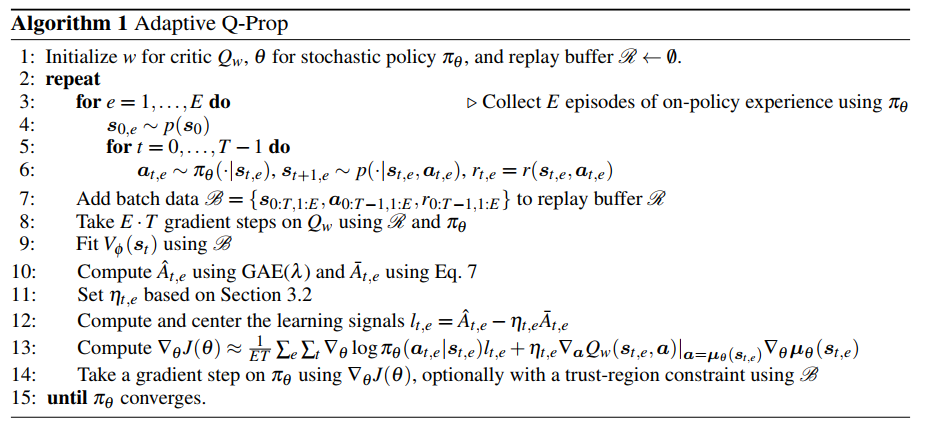
\includegraphics[scale=0.35]{q-prop-algo}
\end{frame}

\subsection{Empirical Results}
\begin{frame}[t]
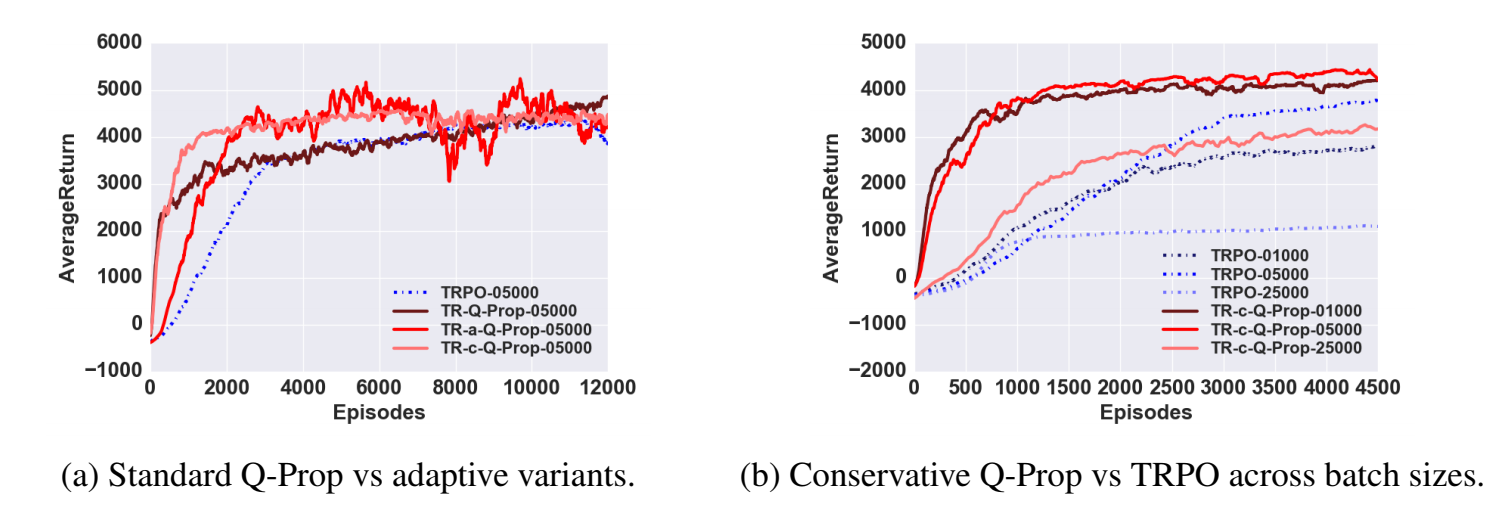
\includegraphics[scale=0.23]{q-prop1}
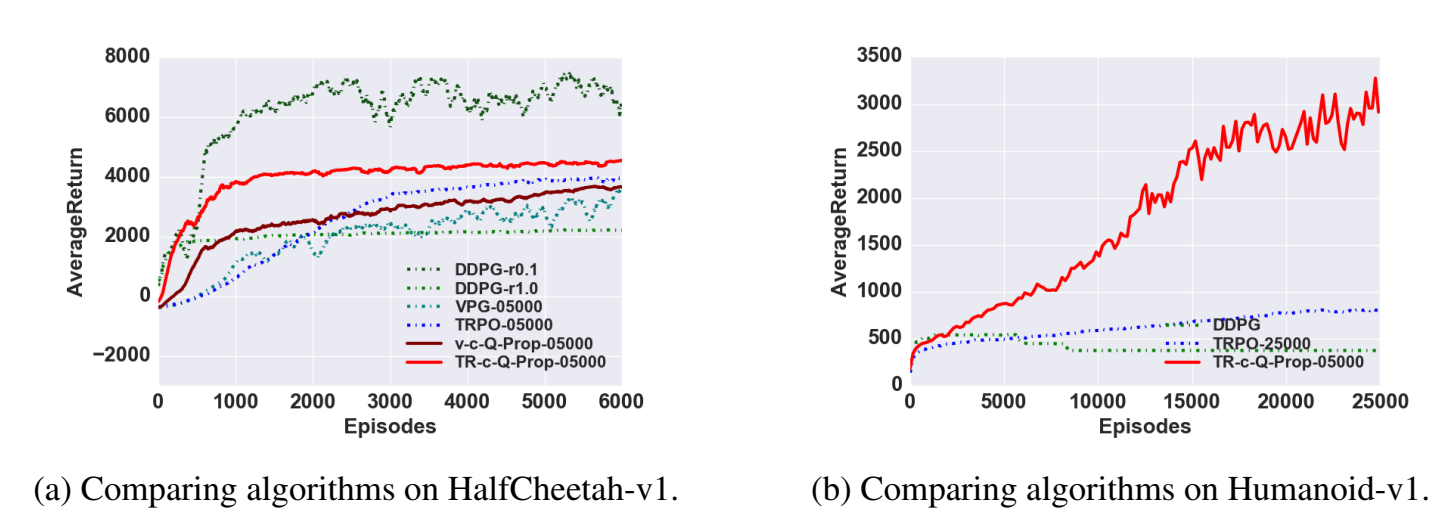
\includegraphics[scale=0.23]{q-prop2}
\end{frame}

\begin{frame}
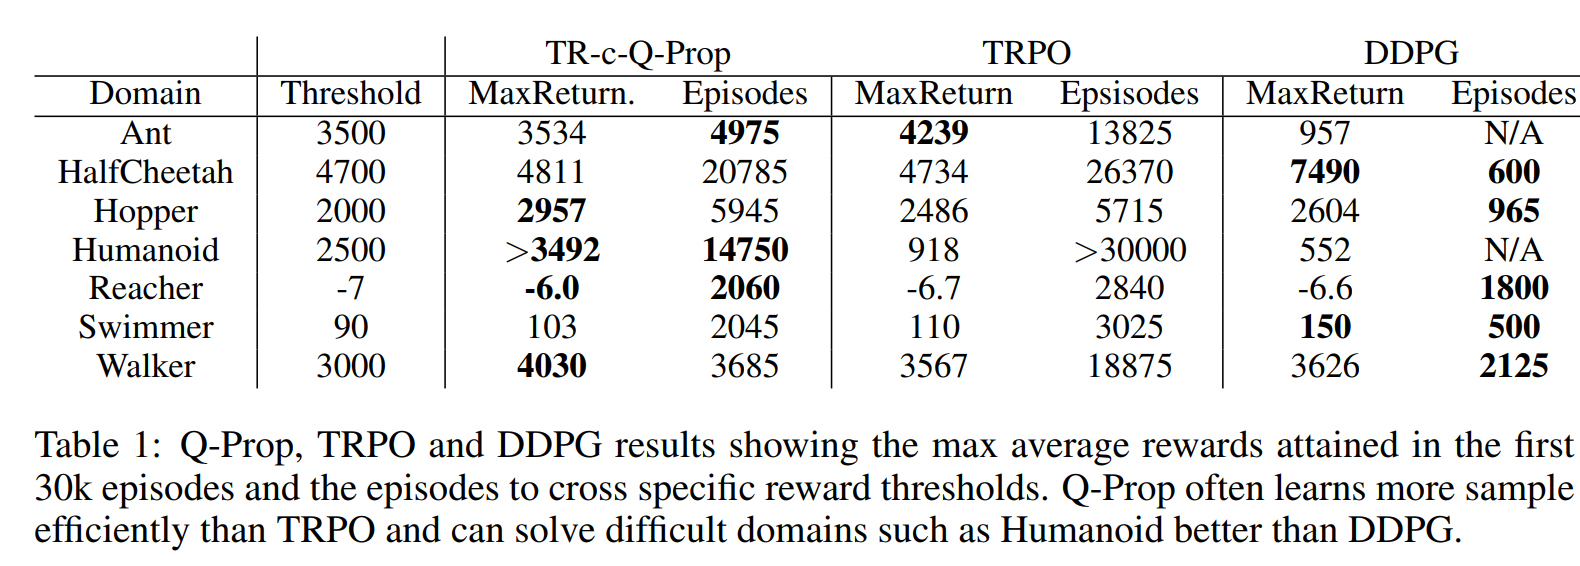
\includegraphics[scale=0.21]{q-prop3}
\end{frame}

\section{Unifying Policy Gradient And Actor-Critic}

\begin{frame}[t]
\frametitle{Unifying Policy Gradient And Actor-Critic}

Proposed extention:
\begin{multline*}
\nabla_{\theta} J \simeq \alpha E_{\rho_\pi, \pi} \left[ \nabla_{\theta} log \pi_\theta ( a_t | s_t) (A(s_t, a_t) - \eta \overline{A_w} (s_t,a_t)) \right] + \\ + \eta E_{\rho_{CR}} \left[ \nabla_a Q_w(s_t, a) |_{a=\mu_\theta(s_t)} 
\nabla_\theta \mu_\theta(s_t)
\right]
\end{multline*}
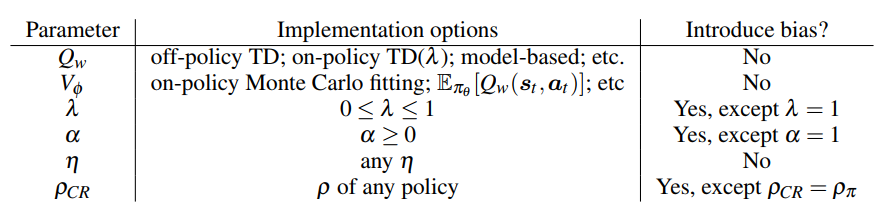
\includegraphics[scale=0.37]{extention}

\end{frame}

\section{RETRACE}


\begin{frame}
\frametitle{Retrace}
Consider Bellman operator:\\
$T_\pi Q (s,a) = r(s,a) + \gamma E_\pi Q(s',a')$\\

\vspace{3mm}
Projection operator:\\
$P_{\Omega, \alpha} Q = argmin_{x \in \Omega} \Vert x - Q \Vert_\alpha$\\

\vspace{3mm}

\begin{itemize}
\item $ \forall \alpha \in [1,\infty], \Vert TQ - TQ' \Vert_\alpha \leq \gamma \Vert Q - Q' \Vert_\alpha, T_\pi Q_\pi = Q_\pi$
\item Then $P_{\Omega, 2} T$ is also a $\gamma$-contraction mapping with supposedly appropriate stationary point
\end{itemize}

\vspace{3mm}
So why bother?

\end{frame}

\begin{frame}[t]
Let:
\begin{itemize}
\item $F$ - $\gamma$-contraction with fixed point $Q^*$\\
\item $Q: \Vert FQ - Q \Vert \leq \epsilon$
\end{itemize}
\vspace{3mm}
Then $\Vert Q^* - Q \Vert \leq \frac{\epsilon}{1-\gamma}$ (use triangle inequality, Luke!)

\vspace{4mm}

Take $F = PT_\pi$;\\
 $\epsilon = \Vert Q_\pi - PQ_\pi \Vert = \Vert Q_\pi - PT_\pi Q_\pi \Vert$ - projection accuracy\\
$\Rightarrow$ for $PT_\pi$'s stationary point $Q^{PT_\pi}$ :
\begin{center}
$\Vert Q^{PT_\pi} - Q_\pi \Vert \leq \frac{\epsilon}{1-\gamma}$
\end{center}

\vspace{4mm}

The upper bound is strict (least upper bound), so for weak contractions the stationary point of $PT_\pi$ can be very far from $Q_\pi$

\end{frame}


\begin{frame}[t]
\frametitle{Retrace}

Consider general form of operator:
\begin{equation*}
R Q (x,a) = Q(x,a) + E_\mu \left[ \sum_{t=0}^\infty \gamma^t \left( \prod_{i=1}^{t} c_t \right) \left( r_t + \gamma E_\pi Q (x_{t+1},.) - Q(x_t,a_t) \right) \right]
\end{equation*}

\begin{itemize}
\item \textbf{IS:} $c_t = \frac{\pi(a_t | s_t) }{\mu(a_t | s_t)}$ \\
Importance Sampling for policy estimation with baseline $Q$. $\forall Q,  R Q = Q_\pi$\\
Yields $Q_\pi$ immediately, though has high variance due to importance sampling

\item \textbf{Q($\lambda$):} $c_t = \lambda$ \\
Let $\epsilon := max_x \parallel \pi(.|x) - \mu(.|x) \parallel _1$, \\
then $\forall \lambda < \frac{1-\gamma}{\epsilon \gamma}$ , $R$ is a contraction 
with fixed point $Q_\pi$\\
Impractical because it's hard to estimate $\epsilon$, low $\lambda$ yields Bellman operator


\end{itemize}
\end{frame}

\begin{frame}[t]

\begin{equation*}
R Q (x,a) = Q(x,a) + E_\mu \left[ \sum_{t=0}^\infty \gamma^t \left( \prod_{i=1}^{t} c_t \right) \left( r_t + \gamma E_\pi Q (x_{t+1},.) - Q(x_t,a_t) \right) \right]
\end{equation*}

\textbf{Retrace($\lambda$):} $c_t = \lambda min \left(1, \frac{\pi(a_t | s_t) }{\mu(a_t | s_t)} \right)$, $\lambda \in [0,1]$\\

\begin{itemize}
\item $\gamma$-contraction around $Q_\pi$.\\ Though we will see a much stronger result in a second\\

\item $\lambda \rightarrow 0 \Rightarrow R \rightarrow T_\pi$\\
Becomes deterministic as $\lambda \rightarrow 0$ - bias-variance tradeoff possibility, though usually unexploited ($\lambda = 1$)

\item "Safe", unlike Q($\lambda$) - defines contraction mapping for any pair of policies, independently of hyperparameters
\end{itemize}

\end{frame}

\begin{frame}
\begin{theorem}
Let $\forall t, 0  \leq c_t \leq \frac{\pi(a_t|s_t) }{\mu(a_t | s_t)}$, then:
\begin{align*}
 \forall \alpha \in  [1, & \infty],\\
& |RQ(x,a) - Q_\pi(x,a)| \leq \eta(x,a) \parallel Q - Q_\pi  \parallel_\alpha
\end{align*}
where $\eta(x,a) := 1 - (1-\gamma) E_\mu \left[ \sum_{t \geq 0} \gamma^t \left( \prod_{i=1}^t c_t \right) \right]$
\end{theorem}

 $\forall t, c_t \simeq 1 \Rightarrow \eta \simeq 0 \Rightarrow R Q \simeq Q_\pi$ - $R$ yields $Q_\pi$ almost immediately if $\mu$ and $\pi$ are close\\
 
\vspace{3mm}
 
\end{frame}

\section{ACER}

\begin{frame}
\frametitle{ACER}
A combination of:
\begin{itemize}
\item RETRACE
\item Stochastic Dueling Networks: simultaneous Q-V off-policy estimation in continuous domain
\item "Trust Region" policy updates for lowering gradient dispersion
\item Importance Sampling with weight truncation and correction
\end{itemize}
\end{frame}

\subsection{Truncation with bias correction}

\begin{frame}
\frametitle{Truncation with bias correction}
 $\nabla J = E_{traj \sim \mu } \left[ \left( \prod_{i=0}^t \rho_i \right) \nabla \log \pi (a_t|s_t) Q(s_t, a_t) | s_0 = s \right]$;
 $\rho_i = \frac{\pi(a_i|s_i)}{\mu(a_i|s_i)}$\\
 \vspace{3mm}
 First, replace full-trajectory importance sampling, involving product of many potentially unbounded weights, with last importance weight $\rho_t$:
 
 \begin{center}
 $\nabla J \simeq g^{marg} = E_{traj \sim \mu } \left[  \rho_t \nabla \log \pi (a_t|s_t) Q(s_t, a_t) \right]$
 \end{center}
  
 \vspace{3mm}
Let $\overline{\rho} = min(c, \rho)$, then:
\begin{align*}
g^{marg} = & E_{traj \sim \mu } \big[ \overline{\rho_t} \nabla \log \pi (a_t|s_t) Q(s_t, a_t) + \\
& + E_{a \sim \pi} \left( \left[\frac{\rho_t(a) - c}{\rho_t(a)}\right]_+ \nabla \log \pi (a|s_t) Q(s_t, a) \right) \big]
\end{align*}
\vspace{3mm}
$\overline{\rho_t}  \leq c$; $\left[\frac{\rho_t(a) - c}{\rho_t(a)}\right]_+ \leq 1$
\end{frame}

\subsection{Stochastic Dueling networks}
\begin{frame}
\frametitle{Stochastic Dueling networks}
Only for estimation in continuous domains
\begin{itemize}
\item Deterministic V estimation
\item Stochastic Q and A estimation
\end{itemize}

\vspace{3mm}
Two "heads": $A, V$
\begin{align*}
\tilde{Q_\omega} (s_t, a_t) \sim & V_\omega (s_t) + A_\omega(s_t, a_t) - \frac{1}{n} \sum_{i=1}^n A_\omega (s_t, u_i),\\ & u_i \sim \pi(.|s_t)
\end{align*}

\begin{itemize}
\item Estimate $V_\omega \simeq V$ is consistent with Q: \\
$E_\pi E_u \tilde{Q_\omega} (s_t, a_t) = V_\omega (s_t)$\\
\item Provides error signal for updating $V_\omega$: $E_u \tilde{Q_\omega} = Q_\pi \Rightarrow V_\omega = E_a E_u \tilde{Q_\omega} = V_\pi$
\end{itemize}

\end{frame}

\subsection{Trust Region updates}
\begin{frame}
\frametitle{Trust Region Updates}
ACER gradient with respect to actor's statistics $\phi_\theta(s_t)$:\\
\begin{align*}
g^{acer} = & \overline{\rho_t}\nabla_\phi log(\pi(a_t|s_t)) \left[ Q^{ret} (s_t,a_t) - V_\theta(s_t) \right] + \\
			& + E_{a \sim \pi} \left[ \frac{\rho_t(a) - c}{\rho_t(a)} \right]_+ \nabla_\phi log(\pi(a|s_t)) [Q_\theta (s_t, a) - V_\theta (s_t)]
\end{align*}

Trust Region:\\

\begin{center}
minimize $\Vert g^{acer} - z \Vert_2$\\
s.t. $k^T z \leq \delta$
\end{center}
\vspace{3mm}
Where:
\begin{itemize}
\item $k = \nabla_{\phi_\theta (s_t)} D_{KL} \left[ \pi_{\phi_{\theta_a}} (s_t) \Vert \pi_{\phi_\theta} (s_t) \right]$\\
\item $\theta_a$ - average policy network
\end{itemize}


\vspace{3mm}
$z^* = g^{acer} - max \left( 0, \frac{k^T g^{acer} - \delta}{\Vert k \Vert_2^2} \right) k$

$z^*$ is then used to calculate gradients with respect to $\theta$ in backpropagation


\end{frame}

\begin{frame}
\begin{center}
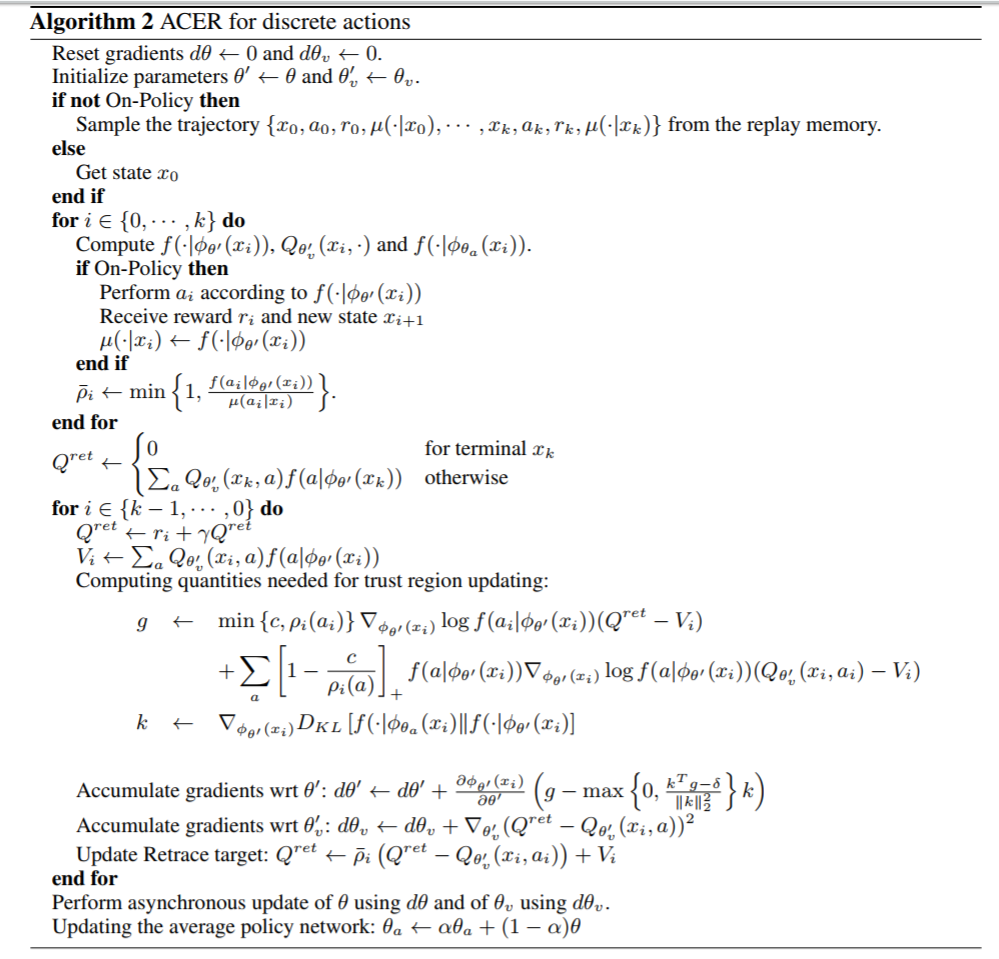
\includegraphics[scale=0.25]{acer_discrete}
\end{center}
\end{frame}

\begin{frame}
\begin{center}
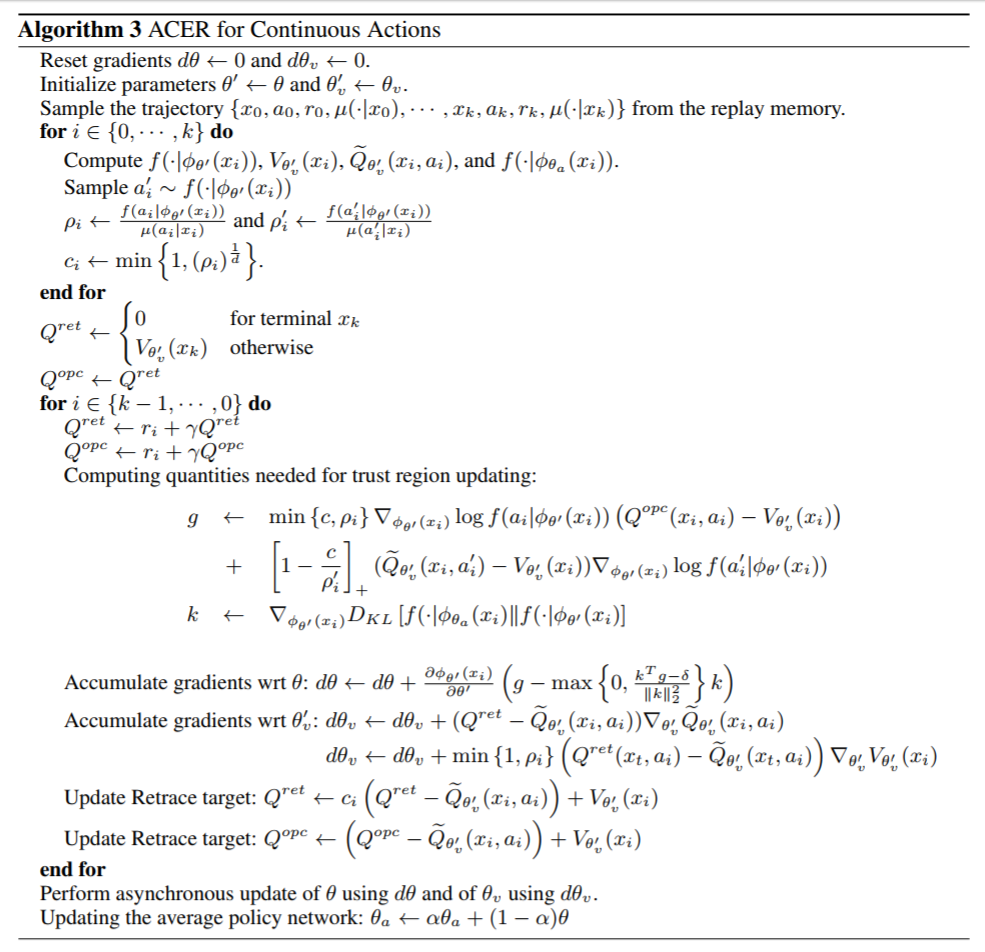
\includegraphics[scale=0.25]{acer_cont}
\end{center}
\end{frame}

\begin{frame}
\frametitle{Ablation analysis}
\begin{center}
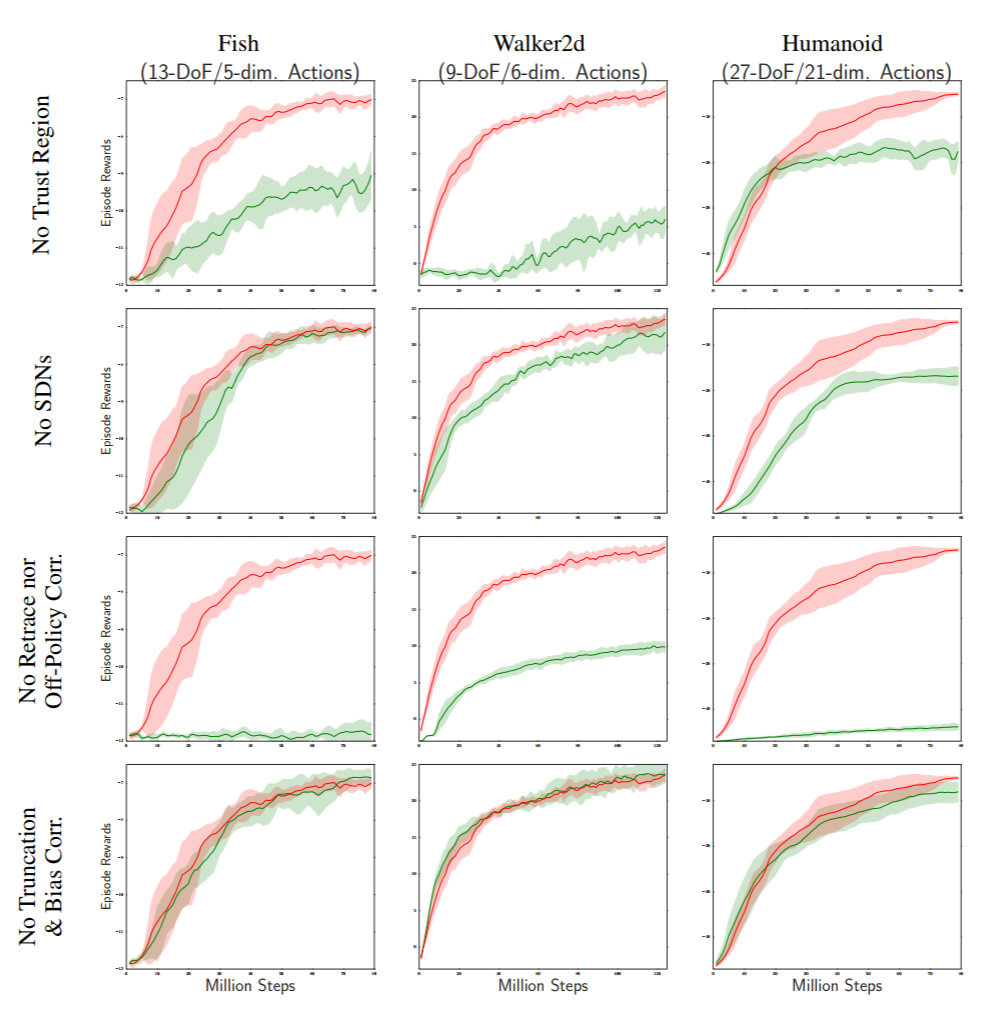
\includegraphics[scale=0.22]{ablation}
\end{center}
\end{frame}

\begin{frame}
\frametitle{Discrete actions}
\begin{center}
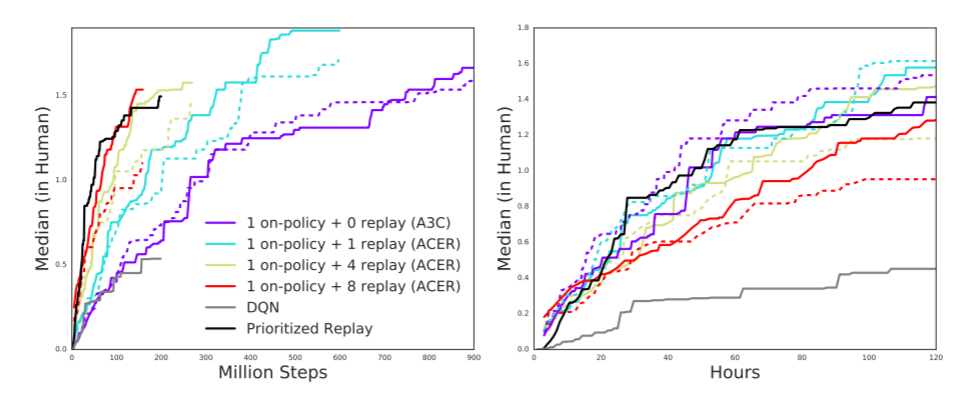
\includegraphics[scale=0.34]{atari}
\end{center}
\end{frame}

\begin{frame}
\frametitle{Continuous actions}
\begin{center}
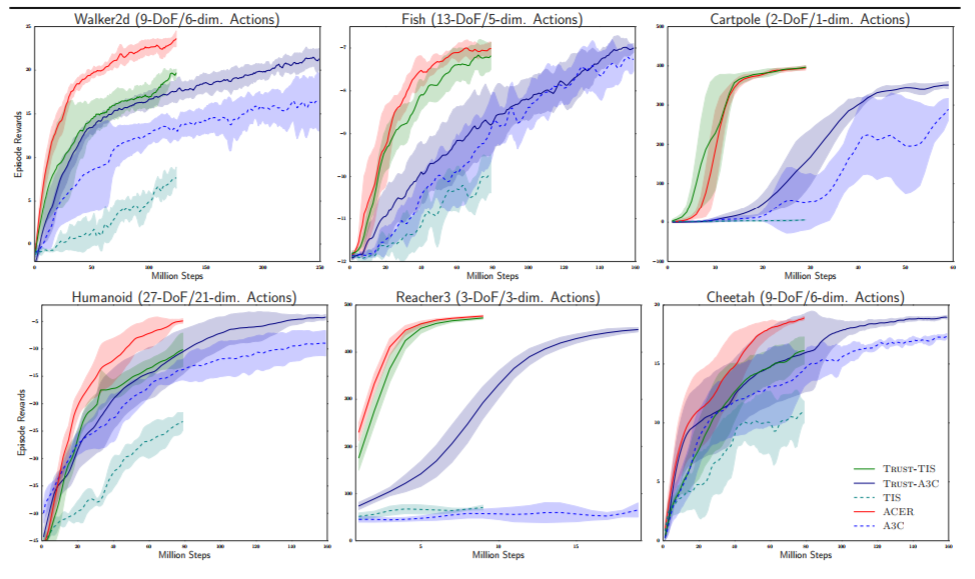
\includegraphics[scale=0.34]{mujoco}
\end{center}
\end{frame}

\end{document}